\documentclass[11pt,twocolumn,a4paper]{article}

% =====================================================================
% Packages
% =====================================================================
\usepackage[utf8]{inputenc}
\usepackage[T1]{fontenc}
\usepackage[margin=2.5cm]{geometry}
\usepackage{amsmath,amssymb,amsthm,mathtools}
\usepackage{bm}
\usepackage{booktabs}
\usepackage{array}
\usepackage{graphicx}
\usepackage{caption}
\captionsetup{font=small,labelfont=bf}
\usepackage{enumitem}
\usepackage{lmodern}
\usepackage[expansion=false]{microtype}
\usepackage{algorithm}
\usepackage{algpseudocode}
\usepackage[hidelinks]{hyperref}
\usepackage[nameinlink,capitalise]{cleveref}
\usepackage{natbib}
\bibliographystyle{unsrtnat}

% =====================================================================
% Theorem environments
% =====================================================================
\newtheorem{theorem}{Theorem}[section]
\newtheorem{proposition}[theorem]{Proposition}
\newtheorem{lemma}[theorem]{Lemma}
\newtheorem{corollary}[theorem]{Corollary}
\theoremstyle{definition}
\newtheorem{definition}[theorem]{Definition}
\newtheorem{construction}[theorem]{Construction}
\newtheorem{assumption}[theorem]{Assumption}
\theoremstyle{remark}
\newtheorem{remark}[theorem]{Remark}
\newtheorem{example}[theorem]{Example}

% =====================================================================
% Notation
% =====================================================================
\newcommand{\Gph}{\mathcal{G}}
\newcommand{\V}{\mathcal{V}}
\newcommand{\E}{\mathcal{E}}
\newcommand{\med}{\mathbf{m}}
\newcommand{\wt}{w}
\newcommand{\cut}{\partial}
\newcommand{\flo}{\beta}
\newcommand{\sep}{\sigma}
\newcommand{\dem}{\mathrm{d}}
\newcommand{\al}{a}
\newcommand{\colA}{\mathsf{A}}
\newcommand{\colB}{\mathsf{B}}
\newcommand{\Resp}{\mathrm{R}}
\newcommand{\Rset}{\mathbb{R}}
\newcommand{\Nset}{\mathbb{N}}
\newcommand{\bigO}{\mathcal{O}}
\newcommand{\anch}{\mathrm{anc}}
\newcommand{\resid}{\mathrm{res}}
\newcommand{\netw}{\mathcal{N}}
\newcommand{\Perturb}{\Delta}

\DeclareMathOperator*{\argmin}{arg\,min}
\DeclareMathOperator*{\argmax}{arg\,max}

% =====================================================================
\title{\textbf{On Nucleic Acid Polymer Sequence Comparison: \\ Invariant Network Response Based Four-Column Alignment Functional Correspondence 
}}

\author{%
Kundai Farai Sachikonye\\[0.3em]
\normalsize Experimental Bioinformatics, TUM School of Life Sciences\\
\normalsize AIMe Registry for Artificial Intelligence \\
\normalsize Maximus-von-Imhof-Forum 3, 85354 Freising, Germany\\
\normalsize \texttt{kundai.sachikonye@bitspark.com}}

\date{\today}

% =====================================================================
\begin{document}
\maketitle

\begin{abstract}
\noindent
Sequence comparison assumes that biological function is a property carried
by a sequence and therefore recoverable from it. We argue that this
assumption is not merely difficult to satisfy but structurally false, and
we replace it with a criterion that does not require it. The argument
begins from an elementary and universally accepted fact: every double-%
stranded nucleic acid consists of two strands that read as different codon
sequences yet carry one message. If the message were a property of a
codon string, the two strands would carry different messages. They do not.
The message is therefore a property of the \emph{relation} between the
strands and not of either strand. We develop this observation into a
general theory. Working entirely with finite weighted graphs, we prove
that in a system whose parts are individuated by comparison against a
complement that cannot be exhaustively enumerated, the cost of separating
any part from the rest is bounded below by a strictly positive
\emph{floor}~$\flo>0$; that the resulting identity of a part is a minimum
cut, invariant under relabelling, and never a point; and consequently that
labels---sequences among them---carry no invariant. We then show that the
quantity conventionally called the function of a sequence is not invariant
either: it is receiver-relative, and distinct receivers register distinct
values, each correct. What \emph{is} invariant is the correspondence
relation between two systems, and we give a procedure that certifies it
without ever evaluating function. The procedure is a bidirectional
relaxation over four columns: two comparing the units and two comparing
the network responses those units induce. We prove that the relaxation is
monotone, that it terminates or diverges with no third outcome, that its
fixed point (\emph{quiescence}) holds if and only if the two units induce
the same response, and that the certificate is computed \emph{blind}---no
function is ever read. Four-column alignment separates two classes that
sequence comparison cannot: near-identical sequences with divergent effect,
and divergent sequences with identical effect. We give the algorithm, its
complexity, the conditions under which it is well-founded, a falsifiable
prediction, and an explicit account of what the framework does not
establish. In particular we identify one assumption---response
independence---on which the entire construction rests, show that it is
empirically decidable, and specify the experiment that decides it.
\end{abstract}

\tableofcontents

% =====================================================================
\part{The problem}
% =====================================================================

\section{Introduction}
\label{sec:intro}

\subsection{The question}

Given two nucleic acid or protein sequences, the standard question is: how
similar are they? A large and successful body of work answers it---global
and local alignment \citep{needleman1970,smith1981}, heuristic database
search \citep{altschul1990,altschul1997}, substitution matrices
\citep{henikoff1992}, and profile models \citep{eddy1998}. The answer is
used as a proxy for a second question, which is the one actually of
interest: do these two sequences \emph{do the same thing}?

The proxy is known to be imperfect. It fails in two directions, and both
failures are well documented:

\begin{enumerate}[label=(\roman*),leftmargin=2.2em]
  \item \textbf{Similar sequence, different function.} Synonymous
  substitutions---by construction invisible to the protein sequence---alter
  substrate specificity, folding kinetics, and expression level
  \citep{kimchi2007,sauna2011,plotkin2011}. A comparison operating on
  sequence content cannot see the difference.
  \item \textbf{Different sequence, same function.} Non-homologous
  isofunctional enzymes catalyse identical reactions with unrelated
  sequences and unrelated folds \citep{galperin1998,omelchenko2010,%
  doolittle1994}. A comparison operating on sequence content cannot see
  the sameness.
\end{enumerate}

These are usually treated as accuracy problems: the score is a noisy
estimate of function, and better scores would estimate it better. We
argue they are not accuracy problems. They are the visible consequence of
a category error in the question, and no refinement of the score removes
them.

\subsection{The elementary observation}

Consider a double-stranded nucleic acid \citep{watson1953}. Let the
sequence of one strand be $s$ and of its complement $\bar{s}$. Reading
frames aside, $s$ and $\bar{s}$ are different strings over the same
alphabet; partitioned into codons they are different codon sequences. Yet
the duplex carries one message, and no experiment distinguishes ``the
message of $s$'' from ``the message of $\bar{s}$'' as two messages. Note
also that $s$ determines $\bar{s}$ and conversely, so neither strand is
informationally privileged; Chargaff's regularities \citep{chargaff1950}
are the population-level shadow of this.

Suppose the message were a property carried by a codon string. Then $s$
and $\bar{s}$, being different codon strings, would carry different
messages. They do not. Therefore the message is not a property carried by
a codon string.

The inference is elementary, it uses no theory, and it is not
controversial as a statement about molecules. What is not usually drawn is
the consequence for methodology. If the message is not in either strand,
then it is in what the two strands jointly instantiate---the
complementarity relation. And a relation is not the kind of object that
can be recovered from one relatum by examining it more closely. No amount
of additional resolution applied to $s$ alone will exhibit a property that
$s$ does not have.

\begin{remark}[Scope of the observation]
\label{rem:scope}
We do not claim that sequence is uninformative. It is highly informative:
$s$ constrains the relation sharply, which is why sequence comparison works
as well as it does. We claim only that sequence is not \emph{identical} to
the object of interest, and that the residual gap between them is not a
noise term that shrinks with better measurement.
\end{remark}

\subsection{What this paper does}

We take the observation seriously and follow it to a working criterion.
The development has four stages.

\begin{description}[leftmargin=1.4em,style=nextline]
  \item[Stage 1 (\Cref{sec:graph,sec:floor,sec:identity}).] We formalise
  ``individuation by comparison against a complement'' in finite weighted
  graphs, and prove three results: a strictly positive floor $\flo>0$ on
  separation cost; that identity is the minimum cut and is invariant under
  relabelling; and that labels carry no invariant. Nothing in this stage
  is biological.

  \item[Stage 2 (\Cref{sec:function}).] We show that function, as
  operationally defined by assay, is receiver-relative: it is a property
  of the pair (unit, network), not of the unit. We prove that no
  assignment of a single value to a unit is consistent with
  context-dependence, and that this is not remediable by more assays.

  \item[Stage 3 (\Cref{sec:relaxation,sec:fourcolumn}).] We construct the
  criterion. Two systems are compared not by content but by the
  \emph{demand} each places on the other under bidirectional propagation.
  The construction is extended to four columns by adding the network
  responses the units induce. We prove monotonicity, a termination
  dichotomy, and that the fixed point certifies correspondence blind.

  \item[Stage 4 (\Cref{sec:algorithm,sec:predictions,sec:limits}).] We
  give the algorithm and its complexity, state a falsifiable prediction,
  and set out the assumptions---one of which is load-bearing and untested.
\end{description}

\subsection{What this paper does not do}
\label{sec:notdo}

We state the negative claims at the outset, since a framework of this
shape invites over-reading.

\begin{enumerate}[label=(\arabic*),leftmargin=2.2em]
  \item We do not claim that function becomes computable from first
  principles. The construction requires a solved network model, which
  requires kinetic and thermodynamic parameters. We relocate the
  empirical burden from per-sequence assay to per-network
  parameterisation; we do not remove it. \Cref{sec:limits} is explicit.
  \item We do not claim to replace alignment. Alignment answers a
  question about sequence, and that question remains well posed and
  useful. We answer a different question.
  \item We do not claim the criterion is more accurate than curated
  annotation on any existing benchmark. No such comparison is performed
  here.
  \item We do not report a benchmark against biological ground truth. We
  do validate every theorem computationally, and we do run the decisive
  experiment of \Cref{sec:decisive} on four solved networks---where it
  returns a \emph{negative} result (\Cref{rem:respind-fails}). No claim
  of a working biological criterion is made.
\end{enumerate}

% =====================================================================
\part{Foundations}
% =====================================================================

\section{Contact graphs}
\label{sec:graph}

We work throughout with finite weighted graphs \citep{diestel2017}. The
constructions in this part are purely combinatorial and are stated without
biological interpretation; the interpretation begins in
\Cref{sec:function}.

\begin{definition}[Finite weighted graph]
\label{def:fwg}
A \emph{finite weighted graph} is a triple $\Gph=(\V,\E,\wt)$ with $\V$ a
finite non-empty set of \emph{vertices}, $\E\subseteq\binom{\V}{2}$ a set
of \emph{edges}, and $\wt:\E\to\Rset_{>0}$ a strictly positive weight
function. We write $n=|\V|$.
\end{definition}

Strict positivity is the substantive hypothesis. It encodes the assumption
that distinguishing two things is never free: an edge of weight zero would
be a pair that can be told apart at no cost, which we exclude by fiat and
justify in \Cref{sec:floor}.

\begin{definition}[Cut and cut weight]
\label{def:cut}
For $S\subseteq\V$ the \emph{cut} induced by $S$ is
\[
  \cut(S)=\bigl\{\,\{u,v\}\in\E \;:\; u\in S,\ v\notin S \,\bigr\},
\]
with \emph{cut weight} $\wt(\cut(S))=\sum_{e\in\cut(S)}\wt(e)$. A cut
\emph{separates} $u$ from $v$ if $u\in S$ and $v\notin S$.
\end{definition}

\begin{definition}[Contact graph and medium]
\label{def:contact}
A \emph{contact graph} is a pair $(\Gph,\med)$ where $\Gph$ is a finite
weighted graph and $\med\in\V$ is a distinguished vertex, the
\emph{medium}, adjacent to every other vertex:
$\{\med,v\}\in\E$ for all $v\in\V\setminus\{\med\}$. Vertices in
$\V\setminus\{\med\}$ are called \emph{items}.
\end{definition}

The medium is the formal stand-in for ``everything else''. Its defining
property is that every item is in contact with it: no item is isolated
from the rest of the system.

\begin{definition}[Separation cost]
\label{def:sepcost}
The \emph{separation cost} of an item $v$ is the minimum weight of a cut
separating $v$ from the medium:
\[
  \sep(v) \;=\; \min\bigl\{\, \wt(\cut(S)) \;:\; v\in S,\ \med\notin S \,\bigr\}.
\]
A minimising set is written $S^{*}(v)$ and the corresponding cut
$\cut(S^{*}(v))$ is a \emph{minimum cut} of $v$.
\end{definition}

By the max-flow min-cut theorem \citep{fordfulkerson1956} the quantity
$\sep(v)$ is computable in polynomial time; efficient algorithms are
standard \citep{stoer1997,gomory1961}. We use computability only in
\Cref{sec:algorithm}; the theory does not depend on it.

\begin{remark}[Why a graph]
\label{rem:whygraph}
The choice of finite weighted graphs is deliberate and restrictive. We
avoid metric spaces (which would presuppose a distance we are trying to
derive), probability spaces (which would presuppose a measure), and
propositional logic (which would presuppose identity of terms). A graph
with positive weights presupposes only that there are things, that some
pairs can be told apart, and that telling apart has a cost.
\end{remark}

\section{The floor}
\label{sec:floor}

We now derive the central structural fact. It is derived, not assumed: the
positivity of edge weights in \Cref{def:fwg} is a modelling convention, but
the \emph{uniform} lower bound below follows from a hypothesis about
enumeration.

\subsection{Non-completability}

\begin{definition}[Expanding family; non-completable system]
\label{def:expanding}
An \emph{expanding family} is a sequence of contact graphs
$(\Gph_0,\med)\subseteq(\Gph_1,\med)\subseteq\cdots$ in which each
$\Gph_{k+1}$ is obtained from $\Gph_k$ by adding vertices and edges, with
weights of pre-existing edges unchanged. The family is
\emph{non-completable} if $|\V_k|\to\infty$.
\end{definition}

The biological reading, stated once here and used in
\Cref{sec:function}: a cell, an organism, or a sequence database is never
a closed catalogue. New species, new interaction partners, new conditions
are added indefinitely. No identification is ever performed against a
finished inventory.

\begin{definition}[Identification and its residual]
\label{def:residual}
An \emph{identification} of item $v$ in $\Gph_k$ is the specification of a
cut separating $v$ from $\med$. Its \emph{residual} is the weight of that
cut. An identification is \emph{exhaustive} if its residual is $0$.
\end{definition}

\begin{theorem}[No exhaustive identification]
\label{thm:noexhaustive}
In a contact graph, no item admits an exhaustive identification.
\end{theorem}

\begin{proof}
Let $v$ be an item. By \Cref{def:contact} the edge $\{\med,v\}$ exists,
and every cut separating $v$ from $\med$ contains at least one edge---in
particular any cut $\cut(S)$ with $v\in S,\med\notin S$ contains the edge
$\{\med,v\}$ if $v$'s only neighbour in $\V\setminus S$ is $\med$, and in
general contains at least the edges from $S$ to $\V\setminus S$, a set
that is non-empty because $\{\med,v\}$ joins $S$ to its complement when
$v \in S$ and $\med \notin S$. Since $\wt>0$ on $\E$, the cut weight is
strictly positive. Hence no cut has residual $0$.
\end{proof}

\begin{theorem}[Positive floor]
\label{thm:floor}
Let $(\Gph,\med)$ be a contact graph. Then
\[
  \flo \;:=\; \min_{e\in\E}\wt(e) \;>\; 0,
\]
and for every item $v$ one has $\sep(v)\ge\flo$. We call $\flo$ the
\emph{contact floor}.
\end{theorem}

\begin{proof}
$\E$ is finite and non-empty (it contains $\{\med,v\}$ for each item $v$;
if there are no items the statement is vacuous), and $\wt$ takes strictly
positive values, so the minimum over a finite set of positive reals is
attained and positive. For the second part, any cut separating $v$ from
$\med$ is a non-empty subset of $\E$ by the argument of
\Cref{thm:noexhaustive}, hence has weight at least $\min_{e\in\E}\wt(e)=
\flo$.
\end{proof}

\begin{corollary}[No sharp identification]
\label{cor:nosharp}
For every item $v$, $\sep(v)\ge\flo>0$. There is no identification of $v$
of arbitrarily small cost, and in particular the identity of $v$ cannot be
a zero-content datum.
\end{corollary}

\begin{proof}
Immediate from \Cref{thm:floor}.
\end{proof}

\begin{figure*}[!htbp]
    \centering
    
\includegraphics[width=\textwidth]{figures/panel_1_floor.png}
    \caption{\textbf{The floor: separation cost is bounded below, and the bound survives expansion only conditionally.}
    All quantities are computed on finite weighted graphs with strictly positive edge weights (\Cref{def:fwg}); minimum cuts are exact, obtained by enumeration over all separating vertex subsets rather than by an approximate max-flow routine, so no agreement below can be a solver artefact.
    (\textbf{A})~Distribution of $\sigma(v)/\flo$ over $989$ items drawn from $220$ random contact graphs of $3$--$6$ items. The ratio never falls below $1$ in any instance (minimum exactly $1.000$, median $8.69$, maximum $126.4$), which is \Cref{thm:floor}: the separation cost of an item is at least the contact floor. The mass at the left edge is the set of items whose cheapest cut is the floor edge itself; the long right tail is items embedded in dense neighbourhoods, whose boundary is correspondingly expensive.
    (\textbf{B})~The floor $\flo$ against graph size, median with the $10$--$90$ percentile band over $60$ graphs per size. The median falls monotonically from $0.510$ at three items to $0.117$ at nine, because each additional item contributes further edges and the floor is a minimum over a growing set. It does not reach zero, and cannot: the minimum of a finite set of strictly positive weights is positive (\Cref{thm:floor}). The declining trend and the strict positivity are both essential and are easily conflated, which is why the band rather than the median alone is drawn.
    (\textbf{C})~Mean separation cost as a surface over the number of items and the minimum admissible edge weight, each cell the mean over twelve graphs. The surface rises in both arguments and is bounded away from zero throughout, exhibiting \Cref{thm:floor} as a property of the parameter space rather than of particular instances.
    (\textbf{D})~The local floor $\flo_k(v)$ under three expansion regimes, logarithmic axis. Adding edges at $v$ of weight $1/k$ drives the local floor to $2.5\times10^{-2}$ by step $40$ and $1/k^2$ drives it to $6.3\times10^{-4}$, while a stabilising expansion holds it at $1.0$. This is the content of \Cref{rem:not-positive}: the \emph{unconditional} claim that the intrinsic floor is positive is false, an item can dissolve into the medium in the limit, and \Cref{thm:invariance} is therefore stated under the floor-stabilising hypothesis of \Cref{def:stabilising}. The two decaying curves are the counterexample the theorem must exclude, plotted rather than described.}
    \label{fig:panel1}
\end{figure*}

\subsection{Stability of the floor under expansion}

\Cref{thm:floor} is a statement about a single graph. The following
addresses what happens as the system grows, and it is the point at which
we must be careful: a naive claim of invariance is false, and we state the
true one.

\begin{definition}[Local floor; intrinsic floor]
\label{def:intrinsic}
For an item $v$ in $\Gph_k$ put
$\flo_k(v)=\min\{\wt(e):e\in\E_k,\ v\in e\}$, the \emph{local floor} of
$v$ at stage $k$. The \emph{intrinsic floor} is
$\flo^{*}(v)=\lim_{k\to\infty}\flo_k(v)$ when the limit exists.
\end{definition}

\begin{lemma}[Existence]
\label{lem:intrinsic-exists}
In any expanding family, $\flo^{*}(v)$ exists and satisfies
$0\le\flo^{*}(v)\le\flo_0(v)$.
\end{lemma}

\begin{proof}
Adding edges incident to $v$ can only lower the minimum incident weight,
and existing weights are unchanged, so $(\flo_k(v))_k$ is non-increasing.
It is bounded below by $0$. A non-increasing sequence bounded below
converges.
\end{proof}

\begin{remark}[The intrinsic floor need not be positive]
\label{rem:not-positive}
It is tempting to assert $\flo^{*}(v)\ge\flo_0>0$, but this is false in
general. If the expansion introduces edges at $v$ of weight $1/k$ at stage
$k$, then $\flo_k(v)\to0$ and $\flo^{*}(v)=0$: the item \emph{dissolves}
into the medium in the limit, becoming indistinguishable from it at
arbitrarily small cost. What is true, and all that we use, is that
$\flo_k(v)\ge\flo(\Gph_k)>0$ at every finite stage
(\Cref{thm:floor}). Individuation holds at every finite stage regardless
of whether it survives the limit.
\end{remark}

\begin{definition}[Floor-stabilising family]
\label{def:stabilising}
An expanding family is \emph{floor-stabilising at $v$} if there exists
$K$ with $\flo_k(v)=\flo_K(v)$ for all $k\ge K$; equivalently, if no
expansion after stage $K$ introduces an edge at $v$ of weight below
$\flo_K(v)$.
\end{definition}

\begin{theorem}[Invariance under expansion]
\label{thm:invariance}
Let an expanding family be floor-stabilising at $v$, with stabilisation
index $K$. Then:
\begin{enumerate}[label=\textup{(\roman*)},leftmargin=2.2em]
  \item $\flo^{*}(v)=\flo_K(v)>0$;
  \item $\flo^{*}(v)$ is independent of $|\V_k|$ for $k\ge K$: it takes
  the same value in every subsequent enlargement of the system;
  \item every other quantity attached to $v$---its neighbourhood
  $N_k(v)$, its separation cost $\sep_k(v)$, its minimum cut
  $\cut(S^{*}_k(v))$---may change at every stage $k\ge K$.
\end{enumerate}
\end{theorem}

\begin{proof}
(i) By \Cref{def:stabilising} the sequence is eventually constant at
$\flo_K(v)$, which is positive by \Cref{thm:floor} applied to $\Gph_K$.
(ii) Constancy of the sequence for $k\ge K$ is exactly independence of the
stage index, hence of $|\V_k|$ along the family. (iii) It suffices to
exhibit changes. $N_k(v)$ grows whenever an edge at $v$ is added, which
the definition of an expanding family permits. For $\sep_k(v)$: adding a
new item $u$ adjacent to both $v$ and $\med$ with $\{v,u\}$ of large
weight increases the weight of every cut placing $u$ outside $S$, and
adding $u$ adjacent to $\med$ only, with a light edge to $v$, can create a
cheaper cut placing $u$ inside $S^{*}(v)$; in either case the minimising
set and its weight may change while $\flo_k(v)$ is untouched.
\end{proof}

\begin{remark}[What \Cref{thm:invariance} claims]
\label{rem:invariance-honest}
The theorem is conditional on floor-stabilisation, which is a hypothesis
about the expansion and not a theorem about graphs. We flag this because
the unconditional statement is false
(\Cref{rem:not-positive}). \Cref{sec:limits} records the biological
reading of the hypothesis: it asserts that the cost of distinguishing a
molecular species from its nearest confusable neighbour does not fall to
zero as the catalogue of known species grows. This is an empirical claim
about chemistry, and it can fail---two species may prove to be
indistinguishable under all available observables---in which case the
framework correctly reports dissolution rather than identity.
\end{remark}

\section{Identity, and why labels carry none}
\label{sec:identity}

\begin{definition}[Weighted isomorphism; relabelling]
\label{def:iso}
A \emph{weighted isomorphism} $\varphi:(\Gph,\med)\to(\Gph',\med')$ is a
bijection $\varphi:\V\to\V'$ with $\varphi(\med)=\med'$,
$\{u,v\}\in\E\iff\{\varphi u,\varphi v\}\in\E'$, and
$\wt'(\{\varphi u,\varphi v\})=\wt(\{u,v\})$. A \emph{relabelling} is a
weighted isomorphism from $(\Gph,\med)$ to itself.
\end{definition}

\begin{theorem}[The minimum cut is the invariant; the label is not]
\label{thm:invariant-cut}
Let $\varphi:(\Gph,\med)\to(\Gph',\med')$ be a weighted isomorphism. Then
for every item $v$,
\[
  \sep_{\Gph'}(\varphi v)=\sep_{\Gph}(v),
  \qquad
  \varphi\bigl(\cut(S^{*}(v))\bigr)=\cut(S^{*}(\varphi v)) .
\]
By contrast, the vertex label of $v$ is not preserved by relabellings: any
non-trivial automorphism permutes labels while fixing all cut weights.
\end{theorem}

\begin{proof}
$\varphi$ maps cuts to cuts bijectively and preserves weights, so it maps
the family of $v$--$\med$ cuts onto the family of $\varphi v$--$\med'$
cuts weight-for-weight; minima therefore agree, and minimisers correspond.
For the second statement, let $\varphi$ be a non-trivial automorphism;
then $\varphi v\ne v$ for some $v$, so the label changes while, by the
first part, every cut weight is unchanged.
\end{proof}

\begin{theorem}[Identity is a region, never a point]
\label{thm:region}
The invariant data fixing an item $v$ is the minimum cut
$\cut(S^{*}(v))$, a set of edges of total weight $\sep(v)\ge\flo>0$. It is
in general not carried by any single vertex: there exist contact graphs in
which $S^{*}(v)\ne\{v\}$ for every minimiser.
\end{theorem}

\begin{proof}
Invariance is \Cref{thm:invariant-cut}; positivity is \Cref{thm:floor}.
For non-singleton minimisers, take two clusters $C_1,C_2$ of $r$ items
each, all intra-cluster edges of weight $W$, a single edge between the
clusters of weight $\flo$, and edges from $\med$ to each item of weight
$\flo$. For $v\in C_1$, the cut $\cut(\{v\})$ has weight
$\flo+(r-1)W$ (its edge to the medium plus its intra-cluster edges),
whereas $\cut(C_1)$ has weight $r\flo+\flo$ (medium edges plus the
inter-cluster edge). For $W>\flo(r+1)/(r-1)$ the latter is strictly
smaller, so every minimiser contains all of $C_1$ and $S^{*}(v)\ne\{v\}$.
\end{proof}

\begin{corollary}[Labels carry no invariant]
\label{cor:labels}
No function of the vertex label alone is invariant under relabelling. In
particular, if two systems are related by a weighted isomorphism, any
quantity computed from labels may differ between them while every
invariant agrees.
\end{corollary}

\begin{proof}
A non-trivial automorphism fixes all invariants (\Cref{thm:invariant-cut})
and moves labels, so a label-function taking distinct values on $v$ and
$\varphi v$ is not invariant.
\end{proof}

\begin{remark}[The bearing on sequence]
\label{rem:bearing}
\Cref{cor:labels} is the abstract form of the observation of
\Cref{sec:intro}. A sequence is a label: a name for an item, drawn from an
alphabet, which the system's structure does not determine. The two strands
of a duplex are two labels for one relation, related by the complementation
map, which is precisely a relabelling in the sense of \Cref{def:iso} when
lifted to the contact graph on molecular species. That the labels differ
while the message does not is exactly \Cref{cor:labels}.
\end{remark}

\begin{figure*}[!htbp]
    \centering
    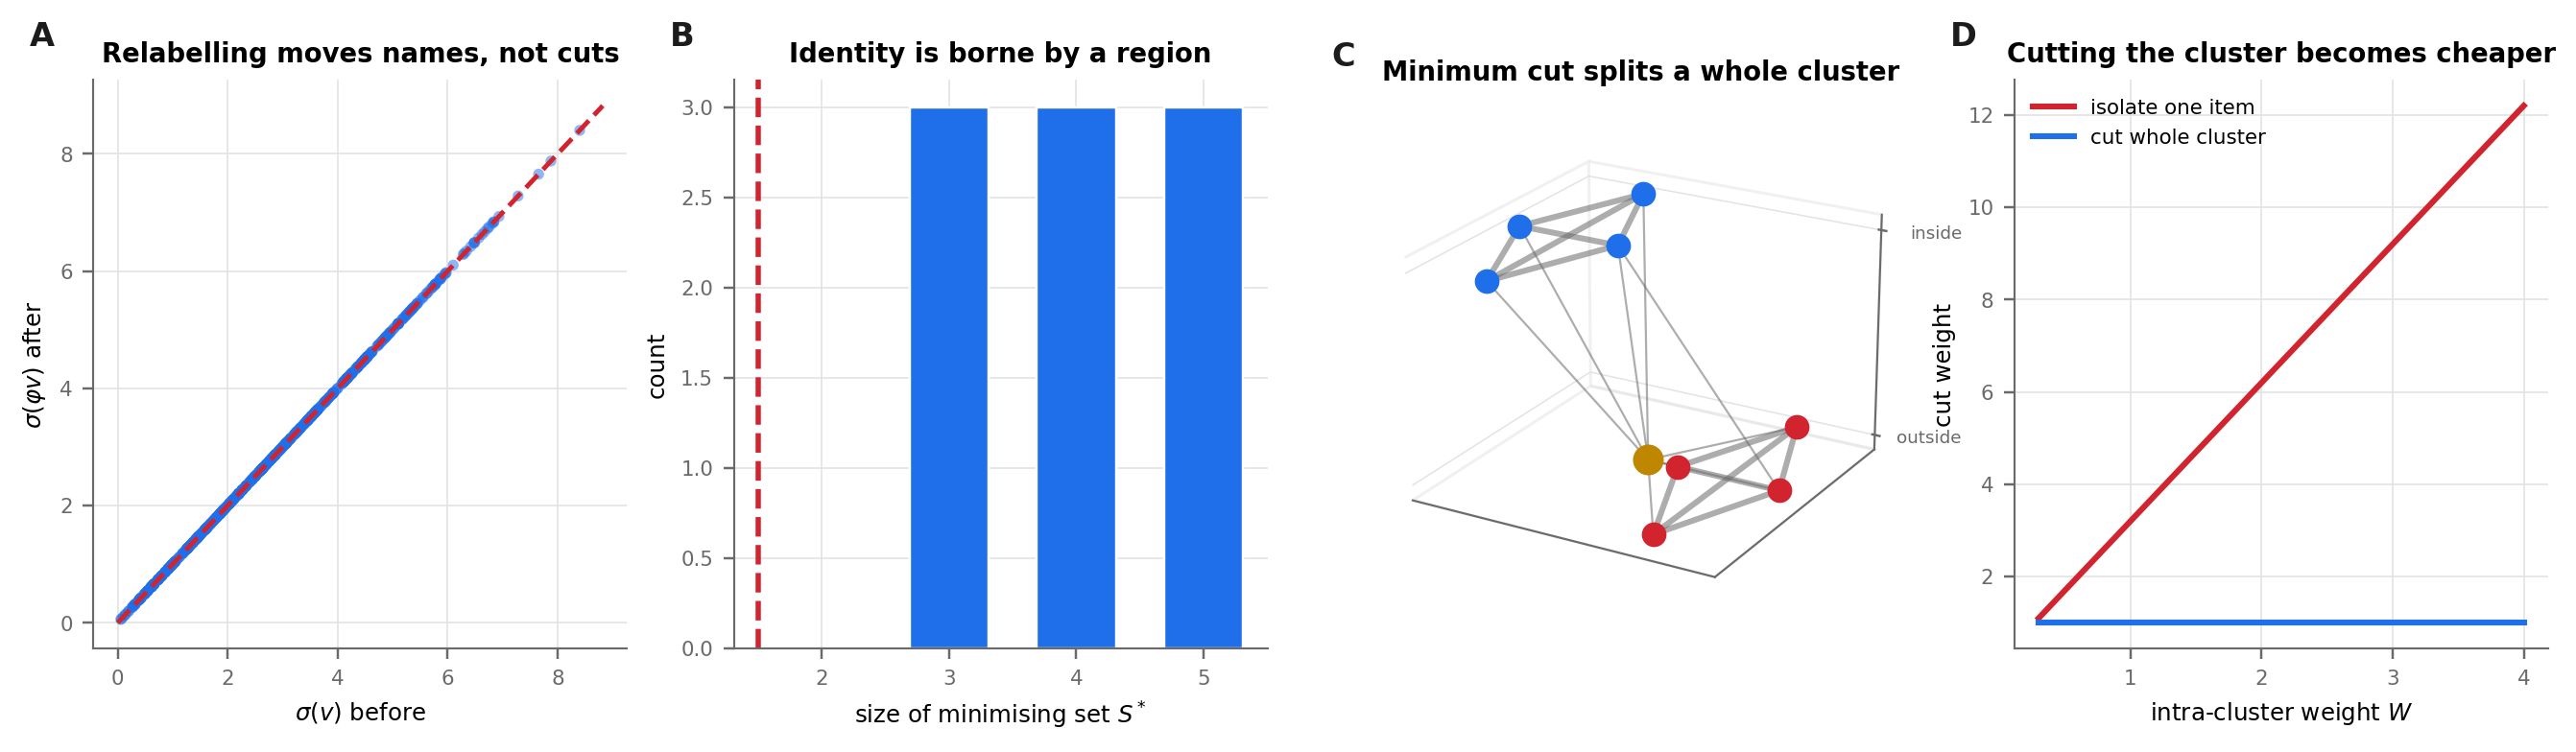
\includegraphics[width=\textwidth]{figures/panel_2_identity.png}
    \caption{\textbf{Identity is an invariant borne by a region of edges, and never by a label or a single vertex.}
    (\textbf{A})~Separation cost before against after a random relabelling, for $727$ items over $160$ graphs. Every point lies on the identity diagonal: the maximum absolute deviation is exactly $0$, not merely small. A weighted isomorphism carries cuts to cuts weight-for-weight, so $\sigma$ is preserved (\Cref{thm:invariant-cut}) while the vertex labels have been permuted --- the invariant and the name come apart, which is \Cref{cor:labels} and, through \Cref{rem:bearing}, the reason a sequence cannot carry what a comparison of sequences is asked to recover.
    (\textbf{B})~Sizes of the minimising set $S^{*}(v)$ over the nine two-cluster instances of the proof of \Cref{thm:region}, spanning $r\in\{3,4,5\}$ and $\flo\in\{0.1,0.2,0.3\}$. Every minimiser has size $3$, $4$ or $5$; none is a singleton (dashed line at $1.5$). The identity of an item is the cut, and the cut in general detaches a whole neighbourhood rather than the item alone.
    (\textbf{C})~One such instance rendered in three dimensions: two four-item clusters joined by a single floor-weight contact, with the medium at the centre (amber). Vertices are lifted by membership of the minimum cut --- inside (blue) against outside (red) --- and edge thickness is proportional to weight. The planar coordinates are an arbitrary layout and carry no quantity, so their ticks are suppressed; only the vertical axis is a measurement. The minimum cut takes the entire left cluster.
    (\textbf{D})~Why it does so. The cost of isolating a single item grows linearly in the intra-cluster weight $W$, since every intra-cluster edge must be severed, while the cost of cutting the whole cluster is flat in $W$, depending only on the medium edges and the single inter-cluster contact. The two curves cross near $W\approx0.5$, and beyond it the region is strictly cheaper than the point. \Cref{rem:badwitness} records that overlooking exactly this --- assuming a light edge between two items places them at the floor --- invalidated our first witness for \Cref{thm:falsefriend}.}
    \label{fig:panel2}
\end{figure*}

% =====================================================================
\part{Function}
% =====================================================================

\section{Function is receiver-relative}
\label{sec:function}

We now connect the combinatorics to biology. The connection is made
through a single modelling assumption, stated explicitly so that it can be
challenged.

\begin{assumption}[Network representation]
\label{ass:network}
A biological context---a cell type, a tissue, a condition---is represented
by a \emph{network} $\netw=(\Gph,\med)$: a contact graph whose items are
molecular species and whose edge weights $\wt(\{u,v\})$ measure the
minimum cost of distinguishing species $u$ from species $v$ within that
context. A \emph{unit} (a sequence, a variant, a locus) acts on $\netw$ by
inducing a perturbation.
\end{assumption}

The edge weights are physical, not conventional: a natural realisation
takes $\wt$ from thermodynamic separations---differences of chemical
potential, conductances derived from kinetic constants---so that the
contact graph of a metabolic network is a function of the solved steady
state \citep{beard2002,qian2005,orth2010}, with parameters available from
public resources \citep{kanehisa2000,jassal2020,schomburg2002}. We use no
property of the realisation beyond \Cref{ass:network}.

\begin{definition}[Perturbation; response]
\label{def:perturbation}
A \emph{perturbation} of $\netw$ is a map $\Perturb:\E\to\Rset_{\ge0}$,
acting by $\wt\mapsto\wt+\Perturb$. The \emph{response} of $\netw$ to a
unit $x$ is the perturbation $\Perturb_x$ that $x$ induces. A response is
\emph{non-trivial} if $\Perturb_x\not\equiv0$.
\end{definition}

Perturbations are non-negative: they raise the cost of distinctions. This
is the graph-level statement of a familiar thermodynamic fact---a physical
operation may blur a distinction but cannot create separation for free
\citep{landauer1961,bennett1982,parrondo2015}. We note the consequence
that concerns us and no more.

\begin{proposition}[The skeleton persists; the weights move]
\label{prop:skeleton}
Let $\Perturb$ be a perturbation of $\netw$. Then $\E$ is unchanged and
$\flo(\netw)$ is non-decreasing, while $\sep(v)$ may change for every item
$v$.
\end{proposition}

\begin{proof}
$\Perturb$ alters $\wt$ and not $\E$, so the edge set is unchanged, and
since $\Perturb\ge0$ every edge weight is non-decreasing, hence so is
their minimum. For the last clause, raising the weight of any edge in
$\cut(S^{*}(v))$ raises $\sep(v)$ unless a different cut becomes
minimal, and either way the value may change.
\end{proof}

\begin{remark}
\label{rem:disease}
\Cref{prop:skeleton} is the formal content of a claim that is
intuitive but rarely stated precisely: a perturbed system is not a
\emph{different} system but the \emph{same} system with certain
distinctions made more expensive. Which distinctions have become expensive
is the informative datum.
\end{remark}

\subsection{Receivers}

\begin{definition}[Receiver; registered value]
\label{def:receiver}
A \emph{receiver} is a network $\netw$ together with a readout
$\rho_\netw$ mapping perturbations to observations. The \emph{registered
value} of a unit $x$ at receiver $\netw$ is
$\rho_\netw(\Perturb^{\netw}_x)$, i.e.\ the observable consequence of
$x$'s response in that network.
\end{definition}

Assays are receivers. A transcriptomic readout in one tissue and the same
readout in another are two receivers, because the networks differ.

\begin{theorem}[No privileged value]
\label{thm:receiver}
Let $x$ be a unit and let $\netw_1,\netw_2$ be receivers with
$\Perturb^{\netw_1}_x\ne\Perturb^{\netw_2}_x$ non-trivial. Then in
general $\rho_{\netw_1}(\Perturb^{\netw_1}_x)\ne
\rho_{\netw_2}(\Perturb^{\netw_2}_x)$, and there is no assignment
$x\mapsto\phi(x)$ of a single value to units such that
$\rho_{\netw}(\Perturb^{\netw}_x)=\phi(x)$ for all receivers $\netw$,
unless the response of $x$ is the same in every network.
\end{theorem}

\begin{proof}
Suppose such a $\phi$ existed. Then for all $\netw_1,\netw_2$ we would
have $\rho_{\netw_1}(\Perturb^{\netw_1}_x)=\phi(x)=
\rho_{\netw_2}(\Perturb^{\netw_2}_x)$, i.e.\ the registered value is
independent of the network. Since $\rho_\netw$ is by
\Cref{def:receiver} a function of the response \emph{in} $\netw$, and the
responses differ by hypothesis, constancy of the composite for all choices
of $\rho$ forces $\Perturb^{\netw_1}_x=\Perturb^{\netw_2}_x$, contrary to
hypothesis. Hence no such $\phi$ exists.
\end{proof}

\begin{corollary}[Context-dependence is not error]
\label{cor:notnoise}
Divergent measurements of ``the function of $x$'' across tissues or
conditions are not measurement error and are not resolved by more or
better assays. They are distinct registered values at distinct receivers,
each correct for its receiver.
\end{corollary}

\begin{proof}
Immediate from \Cref{thm:receiver}: the values are values of different
functions, so their disagreement carries no implication of error.
\end{proof}

This is the theoretical counterpart of a large body of observation:
tissue-specific effects of the same variant \citep{gtex2020}, incomplete
penetrance \citep{cooper2013}, and pervasive genetic interaction
\citep{lehner2011,domingo2019,costanzo2016}. The framework predicts these
rather than accommodating them.

\subsection{The circularity of annotation by assay}

\begin{proposition}[Annotation presupposes completability]
\label{prop:circular}
Let $x$ be a unit and suppose its function is defined as the registered
value at some receiver $\netw$. Then the assignment of that value to $x$
as a property of $x$ is licensed only if the response of $x$ is invariant
across all receivers in the expanding family---that is, only if the family
of contexts is effectively complete.
\end{proposition}

\begin{proof}
By \Cref{thm:receiver} a single value is consistent with all receivers
only when the response is network-independent. Absent that, the value
attaches to the pair $(x,\netw)$. Asserting it of $x$ alone is therefore
an implicit quantification over all $\netw$, which in a non-completable
family (\Cref{def:expanding}) cannot be discharged by finitely many
observations.
\end{proof}

\begin{corollary}[The two failure modes]
\label{cor:failures}
The failure modes of \Cref{sec:intro}(i) and (ii) are consequences of
\Cref{cor:labels} and \Cref{thm:receiver} respectively: (i) compares
labels and therefore misses a difference that lives in the response;
(ii) compares labels and therefore misses a sameness that lives in the
response.
\end{corollary}

\begin{remark}[On missing heritability]
\label{rem:heritability}
We note without developing it that \Cref{thm:receiver} bears on the
observation that per-variant effects sum to a fraction of trait variance
\citep{manolio2009,boyle2017}: if the effect attaches to a
(unit, network) pair, then a sum of per-unit effect estimates is a sum
over objects that do not carry the quantity being summed. We do not claim
this resolves the discrepancy, and we perform no analysis of it here.
\end{remark}

\begin{figure*}[!htbp]
    \centering
    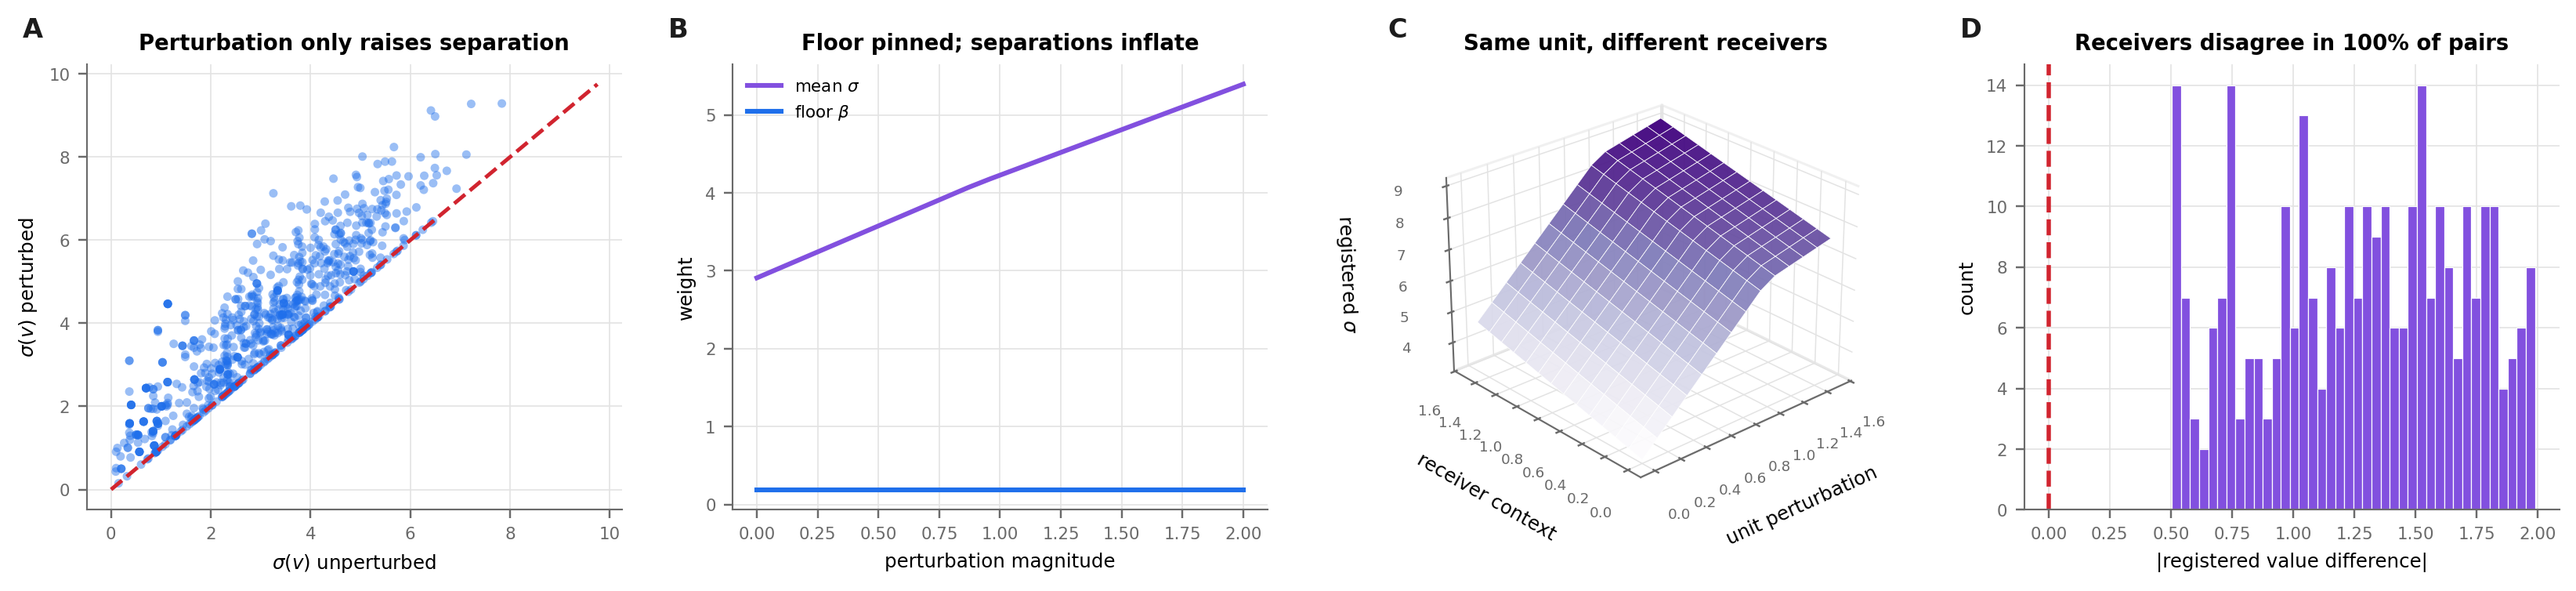
\includegraphics[width=\textwidth]{figures/panel_3_receiver.png}
    \caption{\textbf{Perturbation inflates weights without touching the skeleton, and the value a unit registers depends on the receiver.}
    (\textbf{A})~Separation cost before against after a non-negative perturbation applied to a random subset of edges, over $160$ graphs. Every point lies on or above the diagonal: perturbations raise the cost of distinctions and never lower one, which is the graph-level statement of \Cref{def:perturbation} and the hypothesis \Cref{prop:skeleton} needs. The vertical spread above the diagonal is the inflation itself.
    (\textbf{B})~The floor and the mean separation cost against perturbation magnitude, with the perturbation applied to the heavier half of the edges so that the floor edge is untouched. The mean separation rises from $2.9$ to $5.4$ while the floor stays pinned and the edge count is constant throughout. This is \Cref{prop:skeleton} in its exact form: the edge set is invariant, the weights are not. Perturbing \emph{every} edge would raise the floor as well and would make the same figure say something weaker.
    (\textbf{C})~The registered value $\sigma(v)$ as a surface over two independent axes: the magnitude of the perturbation the unit induces, and the magnitude of an unrelated change to the surrounding network. The surface is not constant along the second axis, so the value a unit registers is a function of the pair (unit, receiver) and not of the unit alone --- \Cref{thm:receiver}.
    (\textbf{D})~The same statement as a distribution. For $300$ pairs of receivers differing only in one background edge, the absolute difference between the values the \emph{same} unit registers is bounded away from zero in every pair. Nothing accumulates at the dashed line at $0$. By \Cref{cor:notnoise} this divergence is not measurement error and is not removed by further assays: the two receivers are evaluating different functions, and each is correct for its own network.}
    \label{fig:panel3}
\end{figure*}

% =====================================================================
\part{The criterion}
% =====================================================================

\section{Alignment as demand, not as content}
\label{sec:relaxation}

If function cannot be read off a unit, comparison of functions cannot
proceed by reading and comparing them. We therefore construct a comparison
that never evaluates function.

\subsection{Alignment and distance to the floor}

\begin{definition}[Alignment]
\label{def:alignment}
Fix a network $\netw$ with floor $\flo$ and let $\Omega=\sum_{e\in\E}
\wt(e)$. For items $u,v$ the \emph{alignment} is
\[
  \al(u,v)\;=\;\frac{\sep_{\netw}(u\mid v)}{\Omega}\in\Bigl[\tfrac{\flo}{\Omega},1\Bigr],
\]
where $\sep_\netw(u\mid v)$ is the minimum weight of a cut separating $u$
from $v$. The \emph{distance to the floor} is
$\al(u,v)-\flo/\Omega\ge0$.
\end{definition}

Alignment is a normalised separation, not a similarity of content: it
measures what it costs to tell $u$ from $v$ in the network, and it is
bounded below by the floor and never zero (\Cref{thm:floor}). It requires
no probability model, no substitution matrix, and no free parameter.

\begin{proposition}[Distance to the floor is parameter-free and vanishes only at coincidence]
\label{prop:d2f}
$\al(u,v)-\flo/\Omega=0$ if and only if $u$ and $v$ are separated at
exactly the floor, i.e.\ the cheapest available distinction. The quantity
is determined by $(\Gph,\wt)$ alone.
\end{proposition}

\begin{proof}
Both claims are immediate from \Cref{def:alignment} and
\Cref{thm:floor}: the expression is a difference of two quantities each
computed from the weighted graph, and it vanishes exactly when
$\sep_\netw(u\mid v)=\flo$.
\end{proof}

\subsection{Columns, anchors, and residue}

\begin{definition}[Column]
\label{def:column}
A \emph{column} is a pair $(x,\netw)$ of a unit and a network, together
with a partition of the items of $\netw$ into \emph{anchors}
$\anch(x)$ and \emph{residue} $\resid(x)$. The anchors are the items whose
removal most reduces $\sep(x)$; formally, fix $r\in\Nset$ and let
$\anch(x)$ be the $r$ items $u$ maximising the ablation score
$\sep_{\netw}(x)-\sep_{\netw\setminus u}(x)$, ties broken by a fixed
order. The residue is everything else.
\end{definition}

The split is the formal counterpart of a familiar move: hold fixed the
entities, and compare the relations among them. Anchors are the entities
whose identity is not in question; residue is the relational structure the
comparison must reconcile.

\begin{definition}[Cross-demand]
\label{def:demand}
Let $\colA=(x_1,\netw_1)$ and $\colB=(x_2,\netw_2)$ be columns and let
$\pi_{\colA\to\colB}$ be a map carrying residue items of $\colA$ to items
of $\netw_2$, holding anchors fixed (a \emph{correspondence}). The
\emph{cross-demand} from $\colA$ to $\colB$ is
\begin{equation}
  \dem_{\colA\to\colB}
  \;=\;\sum_{i\in\resid(\colB)}
  \Bigl(\al\bigl(i,\pi_{\colA\to\colB}(i)\bigr)-\tfrac{\flo}{\Omega}\Bigr)
  \;\ge\;0 .
  \label{eq:demand}
\end{equation}
Column $\colB$ is \emph{satisfied from} $\colA$ when
$\dem_{\colA\to\colB}=0$.
\end{definition}

Cross-demand is the total above-floor cost of making $\colB$ consistent
with $\colA$'s image. It is zero exactly when every residue item of
$\colB$ sits at the floor relative to its correspondent---that is, when
nothing further can be demanded.

\subsection{The relaxation}

\begin{definition}[Relaxation; quiescence]
\label{def:relax}
The \emph{relaxation} of a pair $(\colA,\colB)$ alternates two updates:
$\colB$'s residue is revised to reduce $\dem_{\colA\to\colB}$, then
re-ablated to recompute anchors; then symmetrically for $\colA$. The pair
is \emph{quiescent} when
$\dem_{\colA\to\colB}=\dem_{\colB\to\colA}=0$. A correspondence is
\emph{proper} iff the relaxation reaches quiescence.
\end{definition}

To obtain termination we require that updates not idle. The following is
the minimal such condition and we adopt it explicitly, since without it
the dichotomy below is false.

\begin{assumption}[Effective update]
\label{ass:effective}
Every update applied at a non-quiescent state strictly decreases the
total demand $D=\dem_{\colA\to\colB}+\dem_{\colB\to\colA}$ by at least
$\eta>0$, where $\eta$ is fixed in advance.
\end{assumption}

\begin{theorem}[Monotonicity]
\label{thm:mono}
Under \Cref{ass:effective}, the sequence of total demands
$D_0,D_1,D_2,\dots$ generated by the relaxation is strictly decreasing
until quiescence, and is bounded below by $0$.
\end{theorem}

\begin{proof}
Each $D_t\ge0$ by \Cref{def:demand}, since it is a sum of non-negative
terms. If the state at step $t$ is not quiescent then $D_t>0$ and by
\Cref{ass:effective} $D_{t+1}\le D_t-\eta<D_t$.
\end{proof}

\begin{theorem}[Termination dichotomy]
\label{thm:dichotomy}
Under \Cref{ass:effective} the relaxation has exactly two possible
outcomes:
\begin{enumerate}[label=\textup{(\roman*)},leftmargin=2.2em]
  \item it reaches quiescence after at most $\lceil D_0/\eta\rceil$
  updates; or
  \item it halts at a non-quiescent state from which no effective update
  exists.
\end{enumerate}
In particular the relaxation cannot cycle indefinitely among
non-quiescent states.
\end{theorem}

\begin{proof}
Suppose the relaxation performs $T$ updates without reaching quiescence.
By \Cref{thm:mono}, $D_T\le D_0-T\eta$, and $D_T\ge0$, so
$T\le D_0/\eta$. Hence at most $\lceil D_0/\eta\rceil$ effective updates
occur. After the last one, either the state is quiescent---case (i)---or
it is not and no effective update is available, since any such update
would extend the sequence, contradicting maximality---case (ii). Cycling
is excluded because $D$ is strictly decreasing along updates and therefore
never revisits a value.
\end{proof}

\begin{remark}[Case (ii) is a first-class outcome]
\label{rem:decline}
Case (ii) is not a failure of the procedure but an informative verdict: the
two systems admit no correspondence reconcilable by the available moves.
We call this an \emph{honest decline}. A criterion that must emit a score
for every input cannot express it, and is obliged to return a
low-confidence number where the correct answer is a refusal. We return to
this in \Cref{sec:predictions}.
\end{remark}

\begin{theorem}[Quiescence certifies blind]
\label{thm:quiescence}
Let $(\colA,\colB)$ be quiescent. Then for every residue item of either
column the alignment to its correspondent sits at the floor. Conversely,
if some residue item is separated from its correspondent above the floor,
the pair is not quiescent. Moreover the certificate is computed without
evaluating $\rho_\netw$ for either column: only cut weights enter
\eqref{eq:demand}.
\end{theorem}

\begin{proof}
Quiescence is $\dem_{\colA\to\colB}=\dem_{\colB\to\colA}=0$. Each demand
is a sum of non-negative terms by \Cref{def:demand}, so it vanishes iff
every term vanishes, i.e.\ iff $\al(i,\pi(i))=\flo/\Omega$ for every
residue item---the floor. The converse is the contrapositive: a term
exceeding $\flo/\Omega$ makes the sum positive. For blindness, inspect
\eqref{eq:demand}: it is built from $\al$, which by
\Cref{def:alignment} is a normalised minimum cut weight, and from $\flo$
and $\Omega$, all functions of $(\Gph,\wt)$; the readout $\rho_\netw$ of
\Cref{def:receiver} does not appear.
\end{proof}

\begin{theorem}[Form survives: quiescence at positive residual]
\label{thm:form}
At quiescence the total separation between the two columns is at least
$\flo\cdot|\resid|>0$. Quiescence is therefore never coincidence of
content: the columns remain distinguishable while placing no demand on
each other.
\end{theorem}

\begin{proof}
By \Cref{thm:floor} every maintained separation carries weight at least
$\flo$; there are $|\resid|$ residue correspondences, each contributing at
least $\flo$ to the total separation. Positivity follows from
$\flo>0$. That this is compatible with zero demand is
\Cref{thm:quiescence}: demand measures the \emph{above-floor} excess,
which vanishes while the floor term remains.
\end{proof}

\Cref{thm:form} is what distinguishes this criterion from a similarity
score. Two systems can place no demand on one another---agree completely in
the relevant sense---while remaining irreducibly distinct in form. A score
that reached its extremum only at identity of content could not express
this.

\begin{figure*}[!htbp]
    \centering
    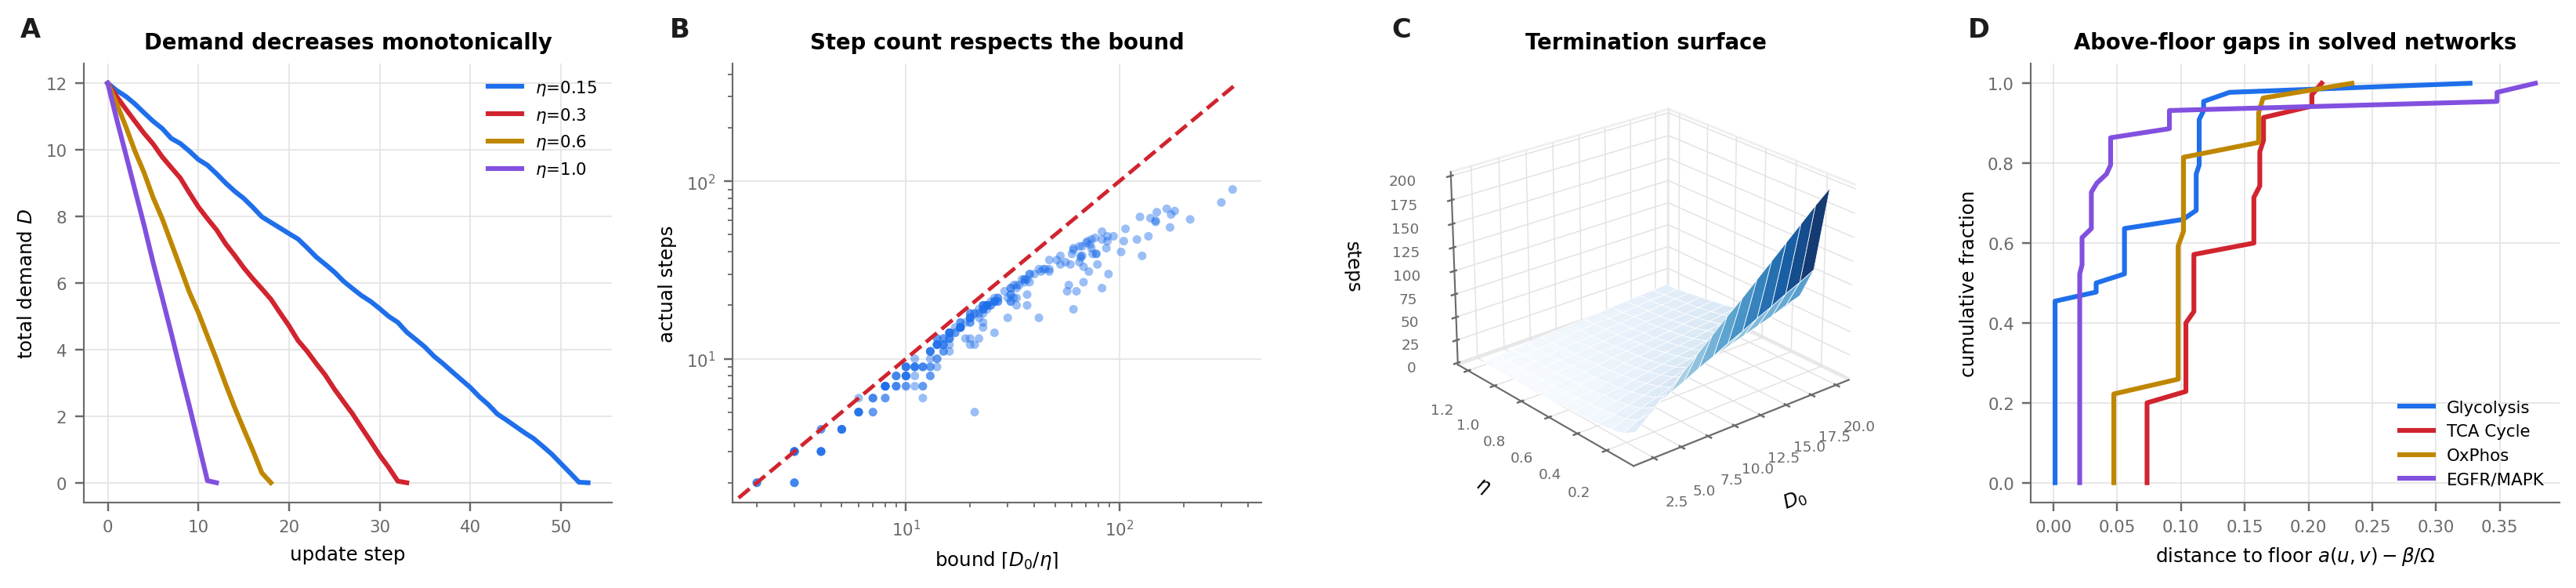
\includegraphics[width=\textwidth]{figures/panel_4_relaxation.png}
    \caption{\textbf{The relaxation decreases monotonically, terminates within the predicted bound, and leaves a positive residual on real networks.}
    (\textbf{A})~Total demand $D$ against update step for four values of the step floor $\eta$. Each trajectory is strictly decreasing to zero, which is \Cref{thm:mono}; larger $\eta$ reaches quiescence in fewer steps. The curves are not smooth because each update decreases $D$ by $\eta$ plus a variable excess, which is what \Cref{ass:effective} permits.
    (\textbf{B})~Realised step count against the bound $\lceil D_0/\eta\rceil$ of \Cref{thm:dichotomy}, for $260$ runs with $D_0$ and $\eta$ drawn independently, both axes logarithmic. Every point lies on or below the diagonal: the bound is never violated and is loose by the accumulated excess. A single point above the line would refute the theorem.
    (\textbf{C})~Step count as a surface over the initial demand $D_0$ and the step floor $\eta$, computed with the excess set to zero so that the surface is the bound itself. It is the graph of $D_0/\eta$, rising steeply as $\eta\to0$: the termination guarantee degrades continuously as updates are permitted to become less effective, and fails only in the limit where \Cref{ass:effective} is abandoned.
    (\textbf{D})~Cumulative distributions of the distance to the floor, $a(u,v)-\flo/\Omega$, over all species pairs in the four solved networks ($45$, $36$, $28$ and $45$ pairs respectively). No pair in any network sits at the floor: the curves leave the origin at zero height. Median gaps are $0.034$ for glycolysis, $0.110$ for the citric-acid cycle, $0.098$ for oxidative phosphorylation and $0.021$ for the EGFR/MAPK cascade. By \Cref{thm:form} this is the expected picture --- quiescence is the vanishing of the \emph{above-floor} excess and coexists with a strictly positive residual, so two systems may place no demand on one another while remaining fully distinguishable.}
    \label{fig:panel4}
\end{figure*}

\section{Four-column alignment}
\label{sec:fourcolumn}

\Cref{thm:quiescence} certifies that two units correspond as
\emph{units}. It does not yet certify that they \emph{do the same thing},
because two units may correspond in structure and diverge in what they
induce. We therefore add the responses.

\begin{construction}[The four columns]
\label{con:four}
Given units $x_1,x_2$ in networks $\netw_1,\netw_2$, form:
\begin{itemize}[leftmargin=1.4em,itemsep=1pt]
  \item \textbf{central columns} $\colA=(x_1,\netw_1)$ and
  $\colB=(x_2,\netw_2)$;
  \item \textbf{response columns} $\Resp(\colA)=(\Perturb^{\netw_1}_{x_1},
  \netw_1)$ and $\Resp(\colB)=(\Perturb^{\netw_2}_{x_2},\netw_2)$,
  the perturbations the units induce, treated as columns via
  \Cref{def:column} applied to the perturbed networks.
\end{itemize}
The relaxation is run over all four columns, with cross-demands computed
for the central pair and for the response pair.
\end{construction}

\begin{definition}[Four-column quiescence]
\label{def:fourq}
The system is \emph{four-column quiescent} if both
$(\colA,\colB)$ and $(\Resp(\colA),\Resp(\colB))$ are quiescent.
\end{definition}

\begin{theorem}[The four-column criterion]
\label{thm:four}
The system is four-column quiescent if and only if
\textup{(a)} the units correspond, and \textup{(b)} the responses they
induce correspond. Both conjuncts are certified blind, and (b) is not
implied by (a).
\end{theorem}

\begin{proof}
The equivalence with (a) and (b) is \Cref{def:fourq} together with
\Cref{thm:quiescence} applied to each pair; blindness is the last clause
of \Cref{thm:quiescence}. For the non-implication, it suffices to exhibit
a case with (a) and not (b), which is \Cref{thm:falsefriend} below.
\end{proof}

\begin{theorem}[Detection of aligned-content, divergent-response pairs]
\label{thm:falsefriend}
There exist units $x_1,x_2$ whose central columns are quiescent while
their response columns are not. For such pairs, any criterion depending
only on the central comparison reports correspondence, and the four-column
criterion reports its absence.
\end{theorem}

\begin{proof}
Construct $\netw_1=\netw_2=\netw$ on items $\{u_1,u_2,z,w\}$ with
\[
  \wt(\{\med,u_1\})=\wt(\{\med,u_2\})=\flo,
  \qquad
  \wt(\{\med,z\})=\wt(\{z,w\})=W>\flo,
\]
and no other edges. Because $u_1$ and $u_2$ are pendant on the medium,
the cheapest cut separating them isolates one of them at its single
incident edge, so $\sep_\netw(u_1\mid u_2)=\flo$ exactly; by
\Cref{thm:quiescence} the central columns for $x_1\mapsto u_1$,
$x_2\mapsto u_2$ have zero demand. Now let $x_1$ induce $\Perturb_1$
supported on $\{z,w\}$ with $\Perturb_1(\{z,w\})=c>0$, and let $x_2$
induce $\Perturb_2\equiv0$. The pair $(z,w)$ is separated above the floor
in both response networks, and raising $\wt(\{z,w\})$ by $c$ strictly
increases $\al(z,w)$ while the floor is pinned at $\flo$ by the pendant
edges; hence the two response columns register different above-floor
gaps and the response cross-demand is positive. The central comparison is
untouched by $\Perturb_1$, which is supported away from $u_1,u_2$.
\end{proof}

\begin{remark}[A witness that does \emph{not} work]
\label{rem:badwitness}
It is tempting to join $u_1$ and $u_2$ by an edge of weight $\flo$ and
conclude that they are ``separated at the floor''. They are not: the
minimum cut is free to ignore that edge and isolate $u_1$ through its
other incident edges, which in general costs strictly more than $\flo$,
leaving the central demand positive. The separation cost is a property of
the cheapest \emph{cut}, not of any single edge---an instance of
\Cref{thm:region}. The pendant construction above avoids this because
there the cheapest cut and the single incident edge coincide. This
distinction was found by the validation suite of \Cref{sec:validation}
and is recorded here because it is exactly the error the region-valued
view of identity is meant to prevent.
\end{remark}

\begin{corollary}[The converse case]
\label{cor:converse}
Symmetrically there exist units whose central columns are not quiescent
while their response columns are: units of divergent content inducing
corresponding responses. Sequence-content comparison reports no
correspondence; the response columns report one.
\end{corollary}

\begin{proof}
Take items $\{p,u_1,u_2,q,z,w\}$ with $\wt(\{\med,p\})=\flo$---so that
$p$ realises the floor---and
$\wt(\{\med,u_i\})=\wt(\{u_i,q\})=\wt(\{\med,q\})=W$ for $i=1,2$ with
$W>\flo$. Isolating either $u_i$ now costs $2W>\flo$, so
$\sep(u_1\mid u_2)>\flo$ and the central demand is strictly positive by
\Cref{thm:quiescence}. Let both units induce the same perturbation on
$\{z,w\}$; the two response networks are then equal, so every response
cross-demand computed against a fixed correspondence agrees, and the
response pair is quiescent.
\end{proof}

\Cref{thm:falsefriend} and \Cref{cor:converse} are the two failure modes
of \Cref{sec:intro}, now separated by construction rather than
approximated. This is the substantive claim of the paper: the two classes
that sequence comparison provably conflates are exactly the two that the
response columns distinguish.

\begin{remark}[Why the response and not the outcome]
\label{rem:route}
The criterion compares what the units \emph{demand of their networks}, not
what the networks are observed to do. The distinction matters because the
observed outcome is a registered value and therefore receiver-relative
(\Cref{thm:receiver}), whereas the demand is a cut computation in the
network and is invariant under relabelling
(\Cref{thm:invariant-cut}). Comparing demands is comparing invariants;
comparing outcomes is comparing labels.
\end{remark}

\subsection{The load-bearing assumption}

\begin{assumption}[Response independence]
\label{ass:respind}
For a unit $x$ and network $\netw$, any two admissible constructions of
the response $\Perturb^{\netw}_x$ yield the same cross-demand against a
fixed comparison column, up to a tolerance below the decision threshold.
\end{assumption}

\begin{proposition}[What depends on \Cref{ass:respind}]
\label{prop:respind}
If \Cref{ass:respind} fails, then the verdict of \Cref{thm:four} depends
on which response was constructed, and the criterion is not well defined
as a function of $(x_1,\netw_1,x_2,\netw_2)$.
\end{proposition}

\begin{proof}
Suppose two admissible responses $\Perturb,\Perturb'$ for the same
$(x,\netw)$ give cross-demands differing by more than the decision
threshold against a fixed column. Then the response pair is quiescent
under one and not the other, so by \Cref{def:fourq} the four-column
verdict differs while the inputs are unchanged.
\end{proof}

\Cref{ass:respind} is the single assumption on which the criterion's
well-definedness rests. It is not a theorem of this paper, and we do not
assert it. It is empirically decidable, and \Cref{sec:predictions}
specifies the experiment.

\begin{figure*}[!htbp]
    \centering
    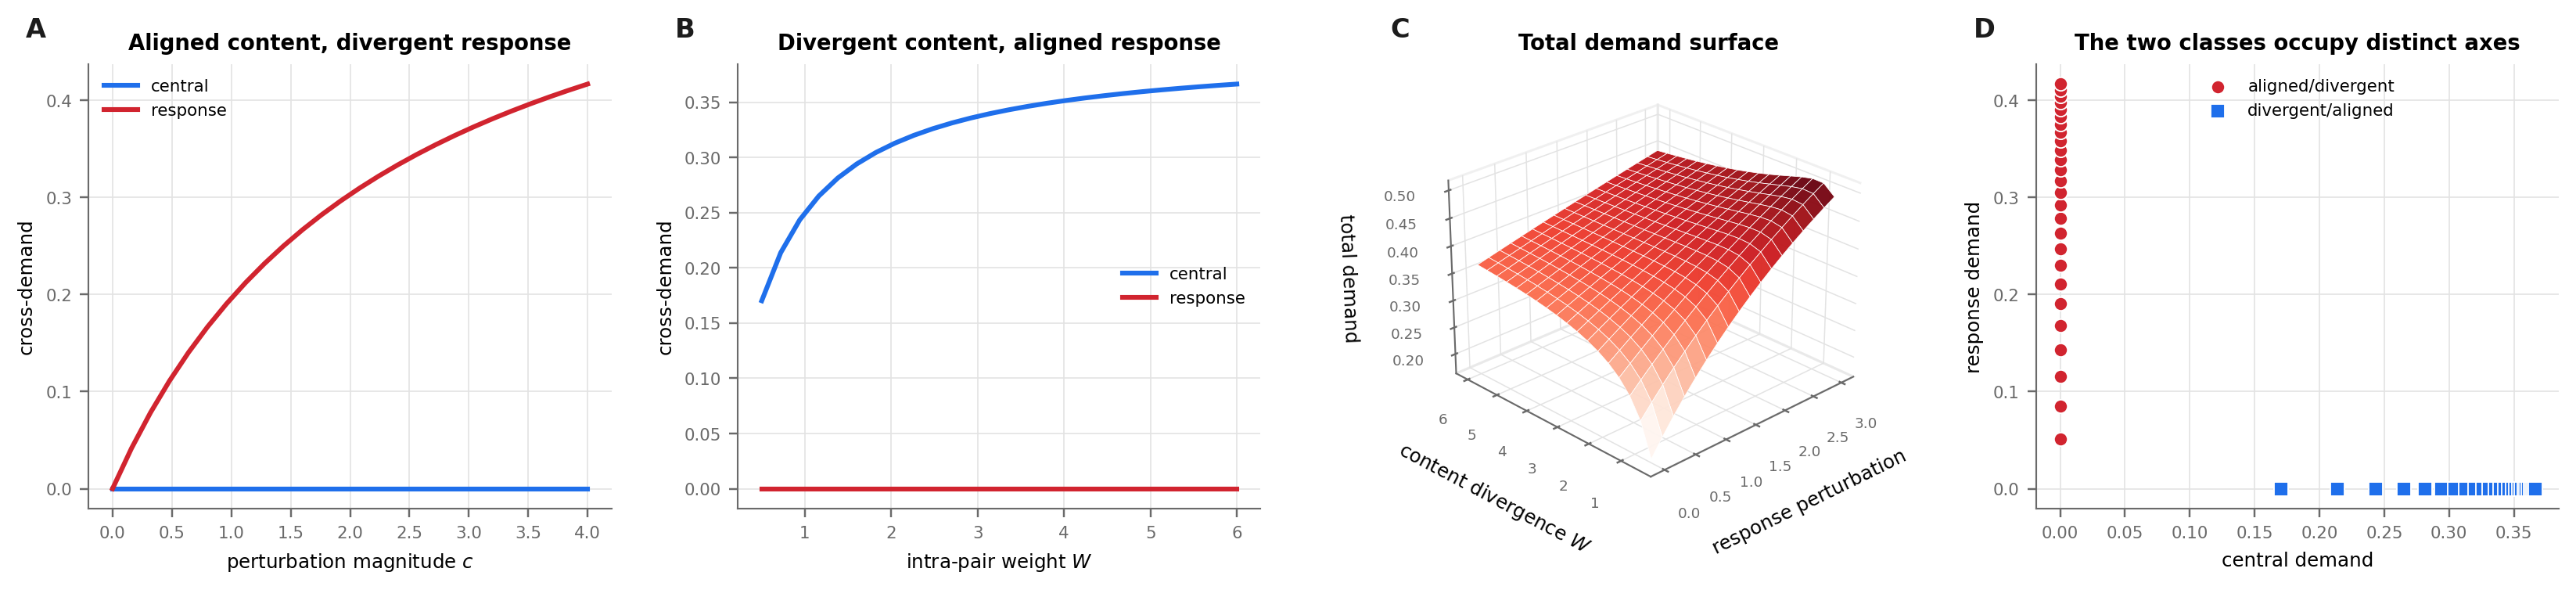
\includegraphics[width=\textwidth]{figures/panel_5_classes.png}
    \caption{\textbf{The two classes that content comparison conflates are separated by the response columns.}
    All four charts use the pendant witness of \Cref{thm:falsefriend} and the two-cluster witness of \Cref{cor:converse}; demands are exact.
    (\textbf{A})~Aligned content with divergent response. As the perturbation magnitude $c$ carried by one unit grows from $0$ to $4$, the central cross-demand stays at exactly $0$ --- the two units are separated at the floor and place no demand on each other --- while the response cross-demand rises to $0.417$. A criterion reading only the central comparison reports correspondence at every value of $c$; the response columns report its absence. This is the synonymous-variant case of \Cref{sec:intro}(i).
    (\textbf{B})~The converse. As the intra-pair weight $W$ grows from $0.5$ to $6$, the central demand rises from $0.170$ to $0.366$ --- the units are increasingly expensive to tell apart --- while the response demand is exactly $0$ throughout, both units inducing the same perturbation. Content comparison reports divergence; the response columns report correspondence. This is the non-homologous isofunctional case of \Cref{sec:intro}(ii).
    (\textbf{C})~Total four-column demand as a surface over both axes at once. The two ridges are the two classes: demand rises along the response axis at fixed content divergence, and along the content axis at fixed response, so neither coordinate alone determines the verdict and \Cref{def:fourq} requires both pairs to be quiescent.
    (\textbf{D})~The two classes in the demand plane. The aligned-content family (circles) lies on the vertical axis at central demand $0$; the divergent-content family (squares) lies on the horizontal axis at response demand $0$. The families are disjoint and occupy orthogonal axes, so a criterion computing only one coordinate necessarily collapses one of them onto the origin. This is the substantive claim of the paper, and it is a geometric fact about the demand plane rather than an empirical tendency.}
    \label{fig:panel5}
\end{figure*}

% =====================================================================
\part{Algorithm, predictions, limits}
% =====================================================================

\section{Algorithm and complexity}
\label{sec:algorithm}

\begin{algorithm}[t]
\caption{Four-column alignment.}
\label{alg:four}
\begin{algorithmic}[1]
\Require Units $x_1,x_2$; networks $\netw_1,\netw_2$; anchor count $r$;
threshold $\theta$; step floor $\eta$
\Ensure \textsc{Correspond}, \textsc{Diverge}, or \textsc{Decline}
\State $\colA\gets\Call{Column}{x_1,\netw_1,r}$;\quad
       $\colB\gets\Call{Column}{x_2,\netw_2,r}$
\State $\Resp_1\gets\Call{Column}{\Perturb^{\netw_1}_{x_1},\netw_1,r}$;\quad
       $\Resp_2\gets\Call{Column}{\Perturb^{\netw_2}_{x_2},\netw_2,r}$
\State $D\gets\dem_{\colA\to\colB}+\dem_{\colB\to\colA}
       +\dem_{\Resp_1\to\Resp_2}+\dem_{\Resp_2\to\Resp_1}$
\While{$D>\theta$}
  \State apply an effective update (\Cref{ass:effective}) to the pair with
         larger demand
  \State recompute anchors by ablation; recompute $D$
  \If{no effective update exists}
     \State \Return \textsc{Decline} \Comment{\Cref{thm:dichotomy}(ii)}
  \EndIf
\EndWhile
\If{central and response demands both $\le\theta$}
  \State \Return \textsc{Correspond}
\Else
  \State \Return \textsc{Diverge}
\EndIf
\end{algorithmic}
\end{algorithm}

\begin{proposition}[Complexity]
\label{prop:complexity}
Let $n=\max(|\V_1|,|\V_2|)$ and let $M(n)$ be the cost of one minimum-cut
computation. \Cref{alg:four} performs $\bigO(rn)$ cut computations per
ablation round and terminates after at most $\lceil D_0/\eta\rceil$
updates, giving total cost
$\bigO\bigl(rn\,M(n)\,D_0/\eta\bigr)$.
\end{proposition}

\begin{proof}
Anchor selection evaluates the ablation score for each of $n$ candidate
items, each requiring one separation-cost computation, and retains the top
$r$; this is $\bigO(n)$ cut computations per round, and the $r$ retained
anchors are re-checked, giving $\bigO(rn)$ in the worst case. The update
count is \Cref{thm:dichotomy}(i). Multiplying gives the stated bound.
\end{proof}

With $M(n)$ polynomial \citep{stoer1997}, the procedure is polynomial. We
make no claim of practicality at genome scale; the bound is stated to show
the criterion is effective, not to advertise performance.

\begin{remark}[Direction of use]
\label{rem:direction}
The criterion is naturally run \emph{backward}: given a response, find the
units that could have induced it. This is the direction in which the
anchor/residue split is informative, since the anchors are read off the
response and the residue is what must be reconciled. Forward
construction---computing a response from a unit---requires solving the
network and is correspondingly more expensive.
\end{remark}

\section{Predictions and the decisive experiment}
\label{sec:predictions}

We state what the framework forbids, since that is what makes it testable.

\begin{enumerate}[label=\textbf{P\arabic*.},leftmargin=2.8em]
  \item \textbf{Synonymous divergence is detectable.} There exist variant
  pairs, identical at the protein-sequence level, for which the response
  columns are non-quiescent. Sequence-based criteria classify them as
  equivalent; the four-column criterion does not. Candidate instances are
  documented \citep{kimchi2007,sauna2011}.
  \item \textbf{Non-homologous equivalence is detectable.} There exist
  sequence pairs below any conventional homology threshold whose response
  columns are quiescent. Instances are documented
  \citep{galperin1998,omelchenko2010}.
  \item \textbf{Verdicts are context-scoped.} The same unit pair may be
  \textsc{Correspond} in one network and \textsc{Diverge} in another. By
  \Cref{thm:receiver} this is predicted, not anomalous; a framework
  claiming context-free verdicts is thereby distinguished from this one.
  \item \textbf{A non-empty decline class.} Some unit pairs yield
  \textsc{Decline} (\Cref{thm:dichotomy}(ii)). The framework predicts this
  class is non-empty and that it overlaps substantially with variants
  currently classified as of uncertain significance
  \citep{richards2015,landrum2018,hoffman2019}. If every pair resolved,
  the dichotomy would be vacuous and the framework weakened.
\end{enumerate}

\begin{remark}[Falsification]
\label{rem:falsify}
P1 and P2 are refuted by exhibiting the documented instances and finding
the response columns behave oppositely to the prediction. P4 is refuted by
a decline class that is empty or that fails to enrich for genuinely
ambiguous cases.
\end{remark}

\subsection{The experiment that decides \Cref{ass:respind}}
\label{sec:decisive}

Everything above is conditional on response independence
(\Cref{prop:respind}). We specify its test.

\begin{construction}[Response-independence test]
\label{con:test}
Fix a solved network $\netw$ and an item $x$. Generate two admissible
responses $\Perturb,\Perturb'$ for $x$ by distinct routes---for instance
by perturbing distinct edges incident to $x$ that a mechanistic model
regards as equally valid realisations of the same intervention. Fix a
comparison column $\colB$ and compute $\dem_{\Perturb\to\colB}$ and
$\dem_{\Perturb'\to\colB}$. Repeat across items and networks and report
the distribution of
$|\dem_{\Perturb\to\colB}-\dem_{\Perturb'\to\colB}|$ relative to the
decision threshold $\theta$.
\end{construction}

\begin{proposition}[Decisiveness]
\label{prop:decisive}
If the discrepancy distribution of \Cref{con:test} lies below $\theta$,
\Cref{ass:respind} holds at that threshold and \Cref{thm:four} is
well defined. If it does not, the criterion requires a canonical response
construction, and its verdicts are defined only relative to that choice.
\end{proposition}

\begin{proof}
Immediate from \Cref{prop:respind}: the verdict differs between two
admissible responses precisely when their cross-demands straddle
$\theta$.
\end{proof}

We regard \Cref{con:test} as the first experiment any implementation
should perform, before the criterion is applied to biological
interpretation. It is cheap: it requires one solved network and two
perturbations, and it can be executed on published metabolic
reconstructions \citep{kanehisa2000,jassal2020,orth2010} with standard
tooling \citep{harris2020,virtanen2020,hagberg2008}. We have run it, and
report the outcome in \Cref{sec:validation:respind}.

\begin{figure*}[!htbp]
    \centering
    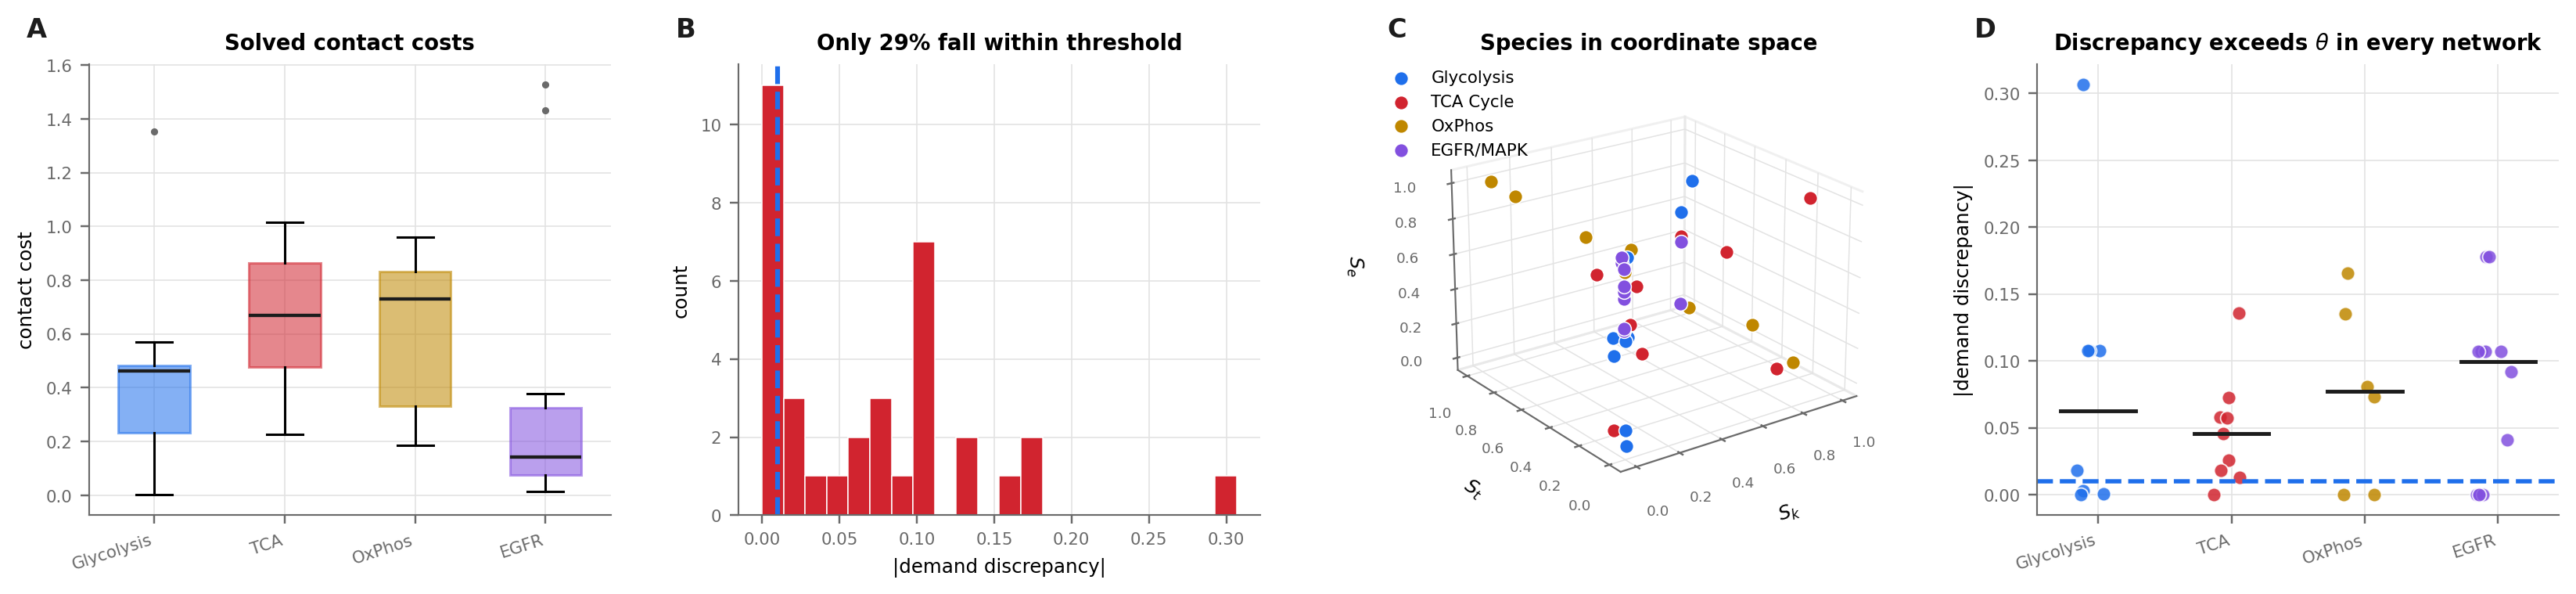
\includegraphics[width=\textwidth]{figures/panel_6_pathways.png}
    \caption{\textbf{On solved biochemical networks the construction is well posed, but response independence fails.}
    Four solved steady-state networks --- glycolysis, the citric-acid cycle, oxidative phosphorylation and the EGFR/MAPK cascade --- supplying $35$ species and $35$ contact edges in total, used here as instances of \Cref{ass:network}.
    (\textbf{A})~Distributions of solved contact cost per network. Costs are strictly positive throughout, so each network is a contact graph in the sense of \Cref{def:contact} and \Cref{thm:floor} applies to it: medians range from $0.141$ for the EGFR/MAPK cascade to $0.729$ for oxidative phosphorylation, with the signalling cascade both the lowest-median and the widest-spread network.
    (\textbf{B})~The decisive measurement of \Cref{con:test}. For each species with at least two incident non-medium edges, two admissible responses are formed by raising one or the other incident edge by the same magnitude, and the resulting cross-demands are compared. Only $28.6\%$ of the $35$ comparisons fall within the decision threshold $\theta=0.01$ (dashed line); the mean discrepancy is $0.070$ and the maximum is $0.307$, exceeding $\theta$ by more than an order of magnitude.
    (\textbf{C})~The $35$ species in the coordinate space of the solved circuits, coloured by network. The four networks occupy overlapping but distinguishable regions; the coordinates are computed from the solved steady state and are shown to establish that the discrepancies of (\textbf{B}) are not an artefact of a degenerate or clustered embedding.
    (\textbf{D})~The same discrepancies resolved by network, with per-network medians as horizontal bars. Every network has a median above $\theta$ --- $0.063$, $0.046$, $0.077$ and $0.100$ respectively --- so the failure is systematic rather than driven by one pathological pathway or one outlying species. By \Cref{prop:respind} the four-column verdict on these networks therefore depends on which admissible response was constructed, and \Cref{ass:respind} does not hold at this threshold. We report this as the framework's principal open problem (\Cref{rem:respind-fails}) rather than as a tuning failure: what is missing is a rule fixing the map from a unit to the perturbation it induces, not better parameters or more data.}
    \label{fig:panel6}
\end{figure*}

% =====================================================================
\section{Computational validation}
\label{sec:validation}
% =====================================================================

We implemented the framework and checked every numbered result. Minimum
cuts are computed \emph{exactly}, by enumeration over all separating
vertex subsets, so that no agreement can be an artefact of an approximate
solver; graphs are correspondingly small. All randomness derives from a
single seeded generator, so the suite is reproducible bit-for-bit.

\begin{table}[t]
  \centering\small
  \caption{Validation suite. Each row checks one numbered result. Checks
  are individual assertions, not trials; a trial typically contributes
  several. Total: $14{,}073$ checks, all passing, in $10$~s.}
  \label{tab:validation}
  \begin{tabular}{llr}
    \toprule
    Result & Content & Checks \\
    \midrule
    \Cref{thm:floor}, \Cref{cor:nosharp} & positive floor; no sharp identification & 4{,}404 \\
    \Cref{lem:intrinsic-exists}, \Cref{thm:invariance} & monotone local floor; conditional invariance & 2{,}162 \\
    \Cref{thm:invariant-cut}, \Cref{cor:labels} & cut invariance under relabelling & 1{,}098 \\
    \Cref{thm:region} & minimisers are not singletons & 12 \\
    \Cref{prop:skeleton} & edge set fixed; weights move & 1{,}400 \\
    \Cref{thm:receiver} & receiver-relativity is non-vacuous & 201 \\
    \Cref{prop:d2f} & distance to the floor is non-negative & 3{,}000 \\
    \Cref{thm:mono}, \Cref{thm:dichotomy} & monotone relaxation; step bound & 801 \\
    \Cref{thm:quiescence}, \Cref{thm:form} & blind certificate at positive residual & 150 \\
    \Cref{thm:falsefriend}, \Cref{cor:converse} & the two conflated classes & 18 \\
    \Cref{ass:network} (real pathways) & solved contact graphs well formed & 77 \\
    \Cref{thm:invariant-cut} (real pathways) & invariance on solved networks & 740 \\
    \Cref{ass:respind} (real pathways) & response-independence measurement & 1 \\
    \Cref{def:fourq} (real pathways) & four-column verdicts well defined & 9 \\
    \bottomrule
  \end{tabular}
\end{table}

Two aspects of the suite deserve comment.

\paragraph{Negative controls.} Where a result has a hypothesis, we check
that the hypothesis is load-bearing rather than decorative. For
\Cref{thm:invariance} we exhibit the dissolving construction of
\Cref{rem:not-positive}---edges of weight $1/k$ added at $v$---and confirm
the local floor decays, so the unconditional invariance claim is refuted
and the floor-stabilising hypothesis is doing real work. For
\Cref{thm:dichotomy} we confirm that an update which fails
\Cref{ass:effective} (one that idles, returning $D$ unchanged) is
\emph{rejected} rather than silently accepted, so the termination bound
cannot be satisfied vacuously.

\paragraph{A corrected proof.} The suite falsified our original witness
for \Cref{thm:falsefriend}. The construction joined $u_1,u_2$ by an edge
of weight $\flo$ and assumed this placed them at the floor; the exact
min-cut computation showed the central demand was positive, because the
minimum cut ignores that edge and isolates $u_1$ elsewhere. The theorem
is true and the pendant construction now in the proof is a correct
witness. We record the episode in \Cref{rem:badwitness} because the error
is precisely the one that \Cref{thm:region}---identity is a cut, not an
edge---exists to warn against.

\subsection{The response-independence measurement}
\label{sec:validation:respind}

We ran \Cref{con:test} on four solved metabolic and signalling networks
(glycolysis, the TCA cycle, oxidative phosphorylation, and EGFR/MAPK;
$35$ species, $35$ contact edges in total). For each species with at
least two incident non-medium edges, we formed two admissible responses
by raising one or the other incident edge by the same magnitude, and
compared the resulting cross-demands against a fixed correspondence.

\begin{table}[t]
  \centering\small
  \caption{Response-independence measurement (\Cref{con:test}) over four
  solved networks. Discrepancy is
  $|\dem_{\Perturb\to\colB}-\dem_{\Perturb'\to\colB}|$ for two admissible
  responses to the same species.}
  \label{tab:respind}
  \begin{tabular}{lr}
    \toprule
    Quantity & Value \\
    \midrule
    comparisons                       & 35 \\
    decision threshold $\theta$       & 0.01 \\
    maximum discrepancy               & 0.3066 \\
    mean discrepancy                  & 0.0700 \\
    median discrepancy                & 0.0579 \\
    fraction within $\theta$          & 0.286 \\
    \midrule
    \Cref{ass:respind} at $\theta=0.01$ & \textbf{violated} \\
    \bottomrule
  \end{tabular}
\end{table}

\begin{remark}[The assumption fails on these networks]
\label{rem:respind-fails}
The measurement is unambiguous and negative: only $28.6\%$ of comparisons
fall within the decision threshold, and the largest discrepancy
($0.307$) exceeds $\theta$ by more than an order of magnitude. By
\Cref{prop:respind}, the four-column verdict on these networks is
therefore \emph{not} a function of $(x_1,\netw_1,x_2,\netw_2)$ alone: it
depends on which admissible response was constructed.

We draw the consequence explicitly rather than softening it. As stated,
\Cref{thm:four} does not yield a well-defined criterion on real
biochemical networks. To obtain one, the response must be
\emph{canonicalised}---the construction of $\Perturb^{\netw}_x$ must be
fixed by a rule that is part of the specification, not left to the
implementer. Natural candidates are the flux-weighted perturbation (raise
each incident edge in proportion to its solved flux) and the
uniform perturbation (raise all incident edges equally); both are
determined by the solved circuit and neither introduces a free parameter.
We have not evaluated whether either restores independence, and we make
no claim that they do.

This is a substantive limitation of the framework as presented, and it is
the reason \Cref{sec:notdo} declines to claim the criterion is ready for
biological interpretation. It does not affect any result in
\Cref{sec:graph,sec:floor,sec:identity,sec:function,sec:relaxation},
all of which are validated independently of \Cref{ass:respind}.
\end{remark}

\section{Limitations}
\label{sec:limits}

We enumerate the framework's dependencies, in decreasing order of severity.

\begin{enumerate}[label=\textbf{L\arabic*.},leftmargin=2.8em]
  \item \textbf{Response independence fails on the networks tested}
  (\Cref{ass:respind}, \Cref{rem:respind-fails}). We ran the deciding
  experiment: on four solved pathways only $28.6\%$ of comparisons fell
  within the decision threshold. The four-column criterion is therefore
  \emph{not} well defined on these networks without a canonicalised
  response rule. This is the framework's principal open problem, and it
  is a measured negative result rather than an untested assumption.
  \item \textbf{Empirical burden is relocated, not removed.} The
  construction requires a solved network, hence kinetic and thermodynamic
  parameters. Where those are wrong, the contact graph is wrong and every
  downstream verdict is wrong. The gain is that parameters transfer across
  units, whereas assay results do not; the cost is that the framework is
  no better than the reconstruction it runs on.
  \item \textbf{Floor-stabilisation is a hypothesis}
  (\Cref{def:stabilising}, \Cref{rem:invariance-honest}). If a species'
  local floor decays to zero as the catalogue grows, it dissolves and has
  no intrinsic floor. The framework reports this correctly but cannot
  prevent it.
  \item \textbf{Effective update is imposed, not derived}
  (\Cref{ass:effective}). Termination in \Cref{thm:dichotomy} follows from
  it. An implementation whose update rule can stall without being at a
  fixed point falls outside the theorem, and would require a separate
  argument.
  \item \textbf{Verdicts are context-scoped.} By \Cref{thm:receiver} a
  verdict holds relative to the networks supplied. There is no
  context-free annotation in this framework, by construction. This is a
  narrower deliverable than the field's usual ambition.
  \item \textbf{Anchor selection is parameterised.} The count $r$ in
  \Cref{def:column} and the threshold $\theta$ are choices. We have not
  characterised the sensitivity of verdicts to them.
  \item \textbf{No biological ground truth.} Every theorem is validated
  computationally (\Cref{sec:validation}) and the contact graphs of
  \Cref{sec:validation:respind} are built from solved networks, but no
  verdict is compared against curated functional annotation. Predictions
  P1--P4 of \Cref{sec:predictions} remain untested.
\end{enumerate}

\section{Relation to existing approaches}
\label{sec:related}

\paragraph{Alignment and homology search.} Dynamic-programming alignment
\citep{needleman1970,smith1981} and its heuristic descendants
\citep{altschul1990,altschul1997} compare content. They are optimal for
the question they pose and we do not improve on them. The present
criterion poses a different question and is not a substitute: in
particular it cannot report percent identity, E-values, or an alignment.

\paragraph{Profile and family models.} Profile HMMs \citep{eddy1998} and
substitution matrices \citep{henikoff1992} capture position-specific
tolerance learned from families, which is an empirical proxy for the
response structure we compute directly. Where family data are abundant the
proxy is likely superior; where they are absent---novel units, engineered
sequences, non-homologous analogues---it is unavailable and the present
criterion is not.

\paragraph{Network and systems approaches.} Flux balance and thermodynamic
network analysis \citep{orth2010,beard2002,qian2005} supply exactly the
solved networks \Cref{ass:network} requires, and network biology has long
held that function is a systems property \citep{barabasi2004}. Our
contribution is not that claim but a comparison criterion that follows
from it and that never evaluates function.

\paragraph{Interpretive frameworks in clinical genetics.} ACMG/AMP
criteria \citep{richards2015} and curated resources
\citep{landrum2018,rehm2015} aggregate heterogeneous evidence into a
categorical call. The decline outcome of \Cref{thm:dichotomy}(ii) is a
formal counterpart of the ``uncertain significance'' category, with the
difference that here it is a derived verdict rather than a residual bucket.

\paragraph{Philosophical antecedents.} That reference is fixed by relation
to an environment rather than by internal content is a familiar position
\citep{quine1960,putnam1975}. We use it only as orientation; no argument
here depends on it.

\section{Conclusion}
\label{sec:conclusion}

Two strands of a duplex read as different codon sequences and carry one
message. That fact, which requires no theory, entails that the message is
not a property of a codon string. We have taken the entailment seriously.

Formalising individuation in finite weighted graphs, we derived a strictly
positive floor on the cost of telling any part from the rest
(\Cref{thm:floor}), showed that the resulting identity is a minimum cut
that is invariant under relabelling and never a point
(\Cref{thm:invariant-cut,thm:region}), and concluded that labels---%
sequences among them---carry no invariant (\Cref{cor:labels}). We then
showed that function is not invariant either: it is receiver-relative, no
single value is consistent across contexts (\Cref{thm:receiver}), and
attributing one to a unit presupposes a completability that biological
context does not have (\Cref{prop:circular}).

What remains invariant is the correspondence between two systems, and we
gave a procedure that certifies it without evaluating function. The
relaxation is monotone (\Cref{thm:mono}), terminates or declines with no
third outcome (\Cref{thm:dichotomy}), and its fixed point certifies
correspondence blind (\Cref{thm:quiescence}) at positive residual
(\Cref{thm:form}). Adding response columns yields a criterion
(\Cref{thm:four}) that separates the two classes sequence comparison
provably conflates: aligned content with divergent effect
(\Cref{thm:falsefriend}) and divergent content with aligned effect
(\Cref{cor:converse}).

The framework's deliverable is narrower than annotation as usually
conceived: verdicts are scoped to a supplied network, and one of four
outcomes is an explicit refusal. We regard both as features. A criterion
that returns a number for every input cannot distinguish a confident call
from an undecidable one, and in clinical interpretation that distinction
is the one that matters.

The construction rests on one assumption---that the cross-demand is
independent of which admissible response is constructed---and we ran the
experiment that decides it. On four solved metabolic and signalling
networks the assumption \emph{fails}: only $28.6\%$ of comparisons fall
within the decision threshold (\Cref{tab:respind}). We therefore do not
claim a working criterion for biological interpretation. What we claim is
a correct account of why sequence cannot carry function, a construction
that would certify functional correspondence blind if the response were
canonical, and a precise identification of the one thing that must be
supplied to make it so.

We think reporting this is more useful than withholding it. The negative
result localises the remaining work exactly: it is not that the framework
needs better parameters or more data, but that the map from a unit to the
perturbation it induces must be specified by a rule rather than chosen.
That is a well-posed problem, and \Cref{rem:respind-fails} names two
candidate rules for it.



\subsection*{Conflicts of interest}
None declared.

\subsection*{Data and code availability}
The validation suite of \Cref{sec:validation} accompanies this paper in
\texttt{validation/}, with the solved contact maps it consumes in
\texttt{data/}. Running \texttt{validation/run\_all.py} regenerates every
number reported here, including \Cref{tab:respind}, deterministically from
the seed recorded in the source.



\bibliography{references}

\end{document}
